\documentclass[titlepage,a4paper]{article}
\usepackage[a4paper,includeheadfoot,margin=2.54cm]{geometry}
\usepackage{graphicx}
\usepackage{listings}
\usepackage{glossaries}
\makeglossaries

\graphicspath{{img/}}
\usepackage{hyperref}
\usepackage{cleveref}

\newcommand\imgwidth{0.5\textwidth}
\newcommand\centrefigurestart{\begin{figure}[h]\begin{center}}
\newcommand\centrefigureend{\end{center}\end{figure}}

\newacronym{sdr}{SDR}{Software Defined Radio}
\newacronym{RF}{RF}{Radio Frequencies}
\newacronym{mitm}{MITM}{man in the middle}
\newacronym{ide}{IDE}{Integrated Development Environment}
\newacronym{vhf}{VHF}{very high frequency}
\newacronym{uhf}{UHF}{ultra high frequency}
\newacronym{gui}{GUI}{graphical user interface}

\begin{document}
\title{Work Experience - RF Guide}
\author{Patrick Mintram}
\maketitle

\tableofcontents
\listoffigures
\printglossaries
\newpage

\section{Introduction}
This guide has been produced to help you work through the \gls{RF} workshop as part of your work experience. In this workshop you will learn \begin{enumerate}\item What things use \gls{RF}. \item How we can make something that uses \gls{RF}. \item How using \gls{RF} can expose your projects to vulnerabilities. \item What tools we can use to help when using \gls{RF}.\end{enumerate}

\subsection{What you will be doing}
In following this workshop you will be using tools available at home, to look at some of the information being sent through the air as \gls{RF}. You will be able to see the different frequencies used by different kinds of devices, such as doorbells, WiFi, remote control cars and bluetooth connected items. You will then send some secret messages between some microcontrollers and use these tools to spy on the message as part of a \gls{mitm} attack.

\subsection{Using this guide}
There may part of this guide which aren't explained very in depth, that is because the subject of \gls{RF} and signals is really complicated, so the detail has been left out. If you want to find out more there are some good overviews available online\footnote{http://www.ti.com/lit/ml/slap127/slap127.pdf, for example}. This guide is meant at more of a practical workshop than an academic exercise, so if something is glossed over a useful link will be provided in the footnotes, as you have already seen. It isn't expected that you full understand the subjects covered, but it is expected that you'll take some time in the future to have a play with the tools and techniques and learn a bit more about the things you've touched on.

\cfbox{red}{ Text in red boxes are things you need to type in. }

\cfbox{blue}{ Text in blue boxes are instructions, but you might not have to type them in. }

\subsection{Feedback}
The author of this guide is keen to know what you think; the good, the bad and the ugly. Please feel free to send any comments their way, or if you're that way inclined, use the github system and raise an issue or create a pull request. 

\newpage

\section{Equipment}
In order to complete this guide you will need the following equipment.

\begin{enumerate}
\item Laptop with the following: 
\begin{enumerate}
\item The \gls{sdr} Drivers. These are usually available from the manufacturers website.
\item The Arduino IDE\footnote{https://www.arduino.cc/en/Main/Software}.
\item The RadioHead-Extras library should be installed and made available to the Arduino IDE. The library is in the \verb|src| folder of this repo.
\item gnuradio\footnote{https://www.gnuradio.org}.
\item A clone of this repo and performed recursively\footnote{git clone --recursive https://github.com/geekskick/wex-guide}.
\end{enumerate}
\item An SDR with an appropriate antenna for looking at the 430-440MHz frequency range. Its up to you which you use, there are loads available for a reasonable price\footnote{https://www.rtl-sdr.com}.
\item Two Adafruit Feathers with an RFM69 packet radio module attached\footnote{https://learn.adafruit.com/adafruit-feather-m0-radio-with-rfm69-packet-radio/overview} as shown in \cref{adafruit}. These should ideally have antennas attached as described in the Adafruit documentation\footnote{https://learn.adafruit.com/adafruit-feather-m0-radio-with-rfm69-packet-radio/antenna-options}. 

\centrefigurestart
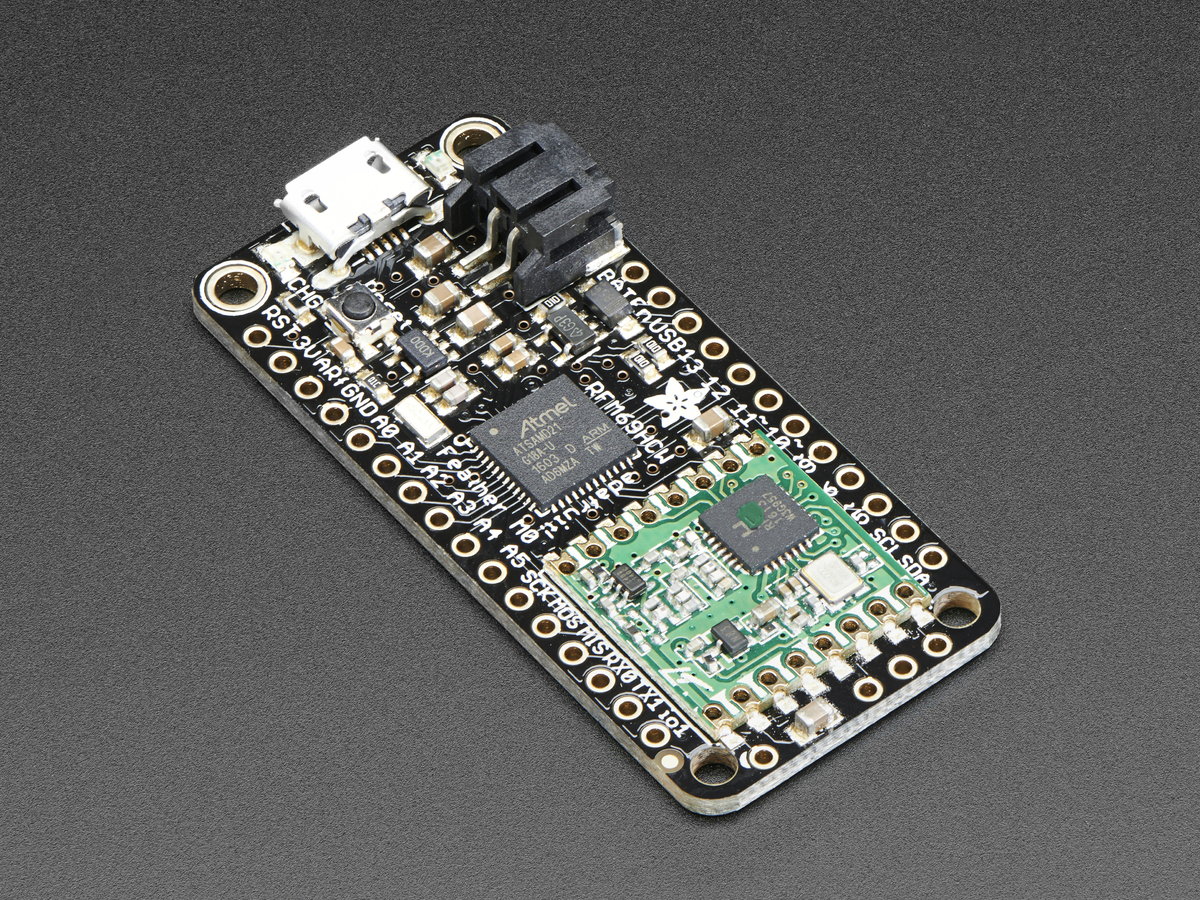
\includegraphics[width=\imgwidth]{feather.jpg}
\caption{An Adafruit Feather M0 with RFM69 Packet Radio}
\label{adafruit}
\centrefigureend

\end{enumerate}
\newpage

\section{Looking at the Spectrum}
The first thing we need to understand is what the \gls{RF} spectrum looks like. There are plenty of electromagnetic waves around, which you may or may not be aware of. Let's quickly revise what a wave looks like, by looking at \cref{wave}\footnote{\url{https://www.bbc.com/bitesize/guides/zgf97p3/revision/1}}.

\centrefigurestart
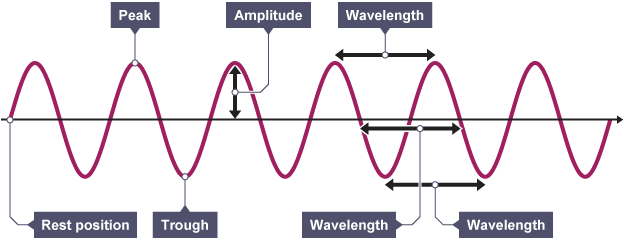
\includegraphics[width=\imgwidth]{bitesize_Wave.png}
\caption{The RF spectrum}
\label{wave}
\centrefigureend

The key thing we care about from this diagram is the wavelength because that determines how long it takes for the wave to happen; it's period. This can be used to calculate how many times it' repeats in a second, this is measured in \textit{Hertz} and is a result of the equation shown in \cref{equ:freq}. 

\begin{equation}
\text{Frequency (Hz)} = \frac{1}{\text{Time for one cycle of the wave (s)}}
\label{equ:freq}
\end{equation}

For example a signal that repeats every 2.309469 nanoseconds has a frequency of 434MHz - it repeats 434 million times a second. There are loads of different frequencies in the \gls{RF} spectrum and 434MHz fits in the \gls{uhf} part of this, as shown in \cref{spectrum}\footnote{\url{https://www.ecnmag.com/blog/2017/06/understanding-rf-spectrum}}.

\centrefigurestart
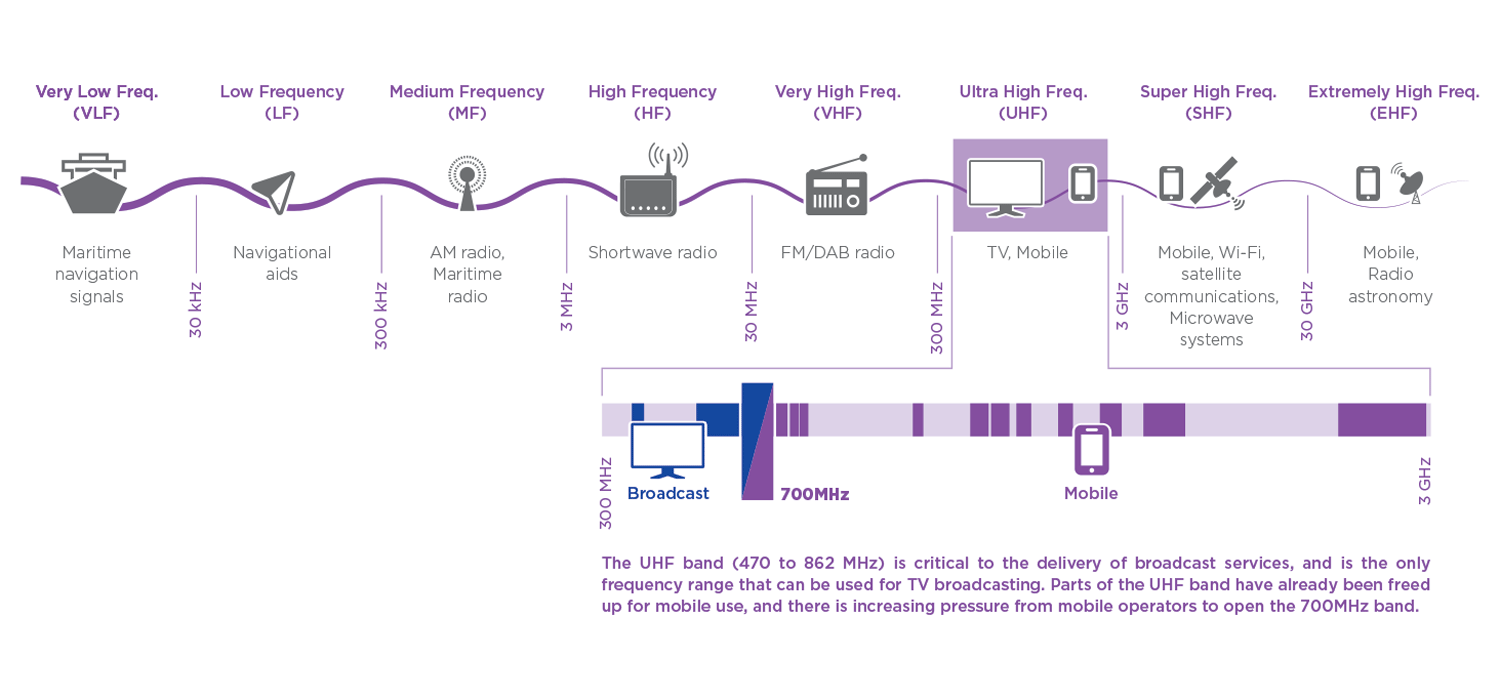
\includegraphics[width=\textwidth]{spectrum_range_services_infographic.png}
\caption{The RF spectrum}
\label{spectrum}
\centrefigureend

We can easily see the effect of these signals by using equipment which uses them; if our radio doesn't work then we know that the signals aren't present at ~90MHz. What about if we want to see a signal at 434MHz though? The radios in our car only tune into parts of the \gls{vhf} frequencies so we can't use those. Here is where our \gls{sdr} comes in useful because we can tell it a frequency to tune into (centre frequency) and we can tell it how quickly to process data (sample rate). We can then plug this into the gnuradio software to see on a graph which frequencies are most powerful, as seen in \cref{uhd_fft}.

\centrefigurestart
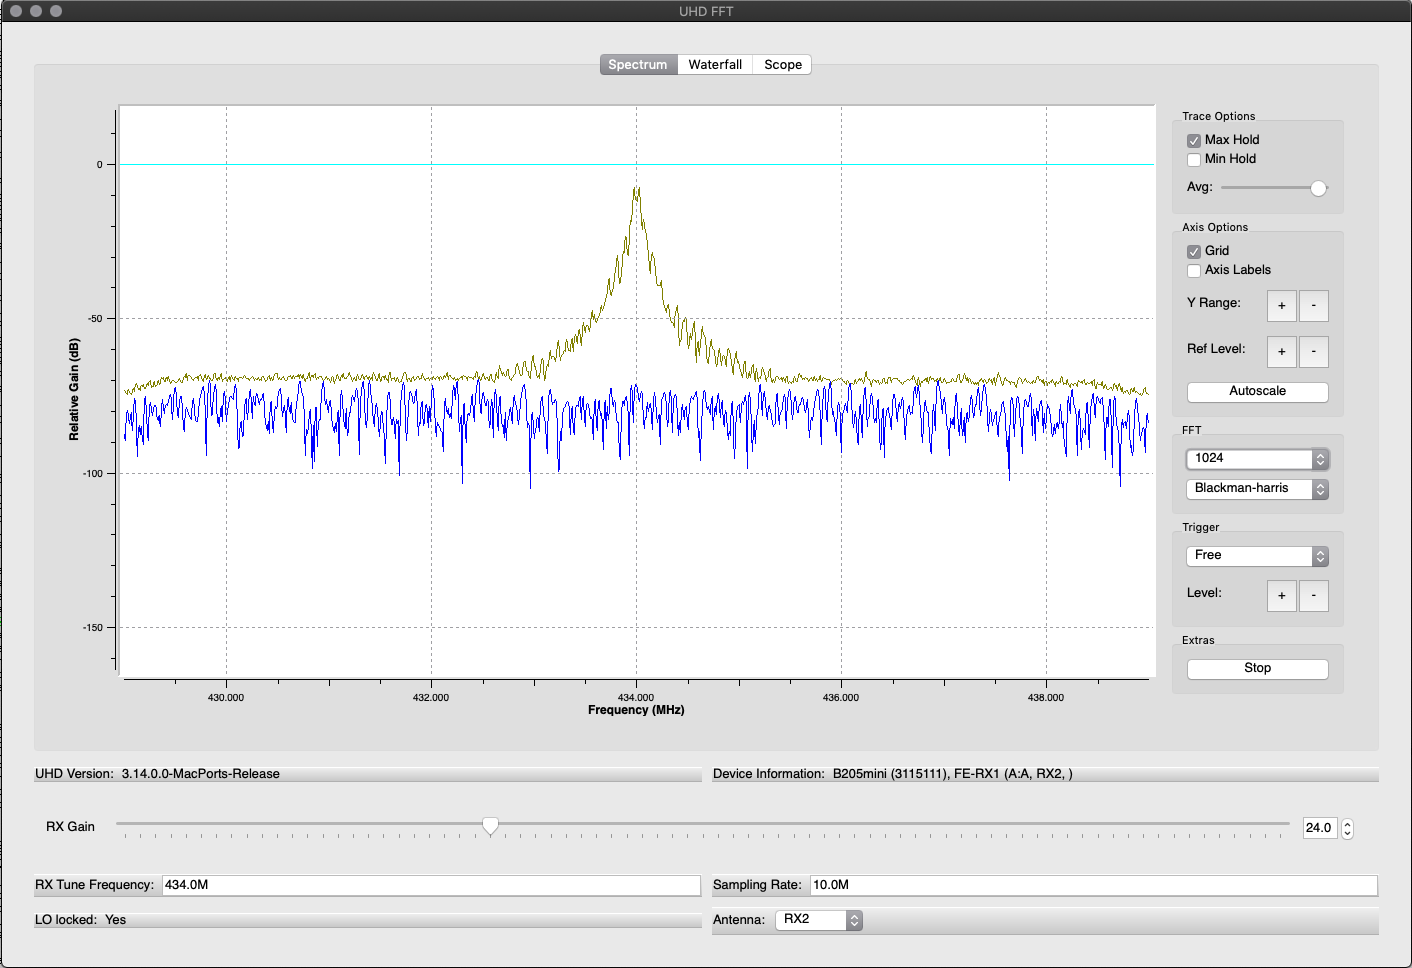
\includegraphics[width=\textwidth]{uhd_fft.png}
\caption{The output of the uhd\_fft command with a 434MHz signal present.}
\label{uhd_fft}
\centrefigureend

The spike on the yellow line in \cref{uhd_fft} shows that there is some signal present at the 434MHz frequency. We can change the settings on this window to see other signals which might be present, but first you need to run the following command from the command line to open the window.
\begin{lstlisting}
uhd_fft -f 434000000 -s 10000000
\end{lstlisting}
Try looking somewhere around 2.4GHz and seeing how busy it is. What do you think these signal might be?

\subsection{gnuradio flows}
Rather than using a prepackaged command like uht\_fft we can make our own \gls{gui}s using gnuradio companion. This can be a bit weird, so to start you off one has been provided. From the command line enter:
\begin{lstlisting}
gnuradio-companion 
\end{lstlisting}
From here open up the provided file FFT.grc and you can click the play button highlighted in \cref{grc_fft} and see the spectrum as we did before. At this point it's worth taking some time to familiarise yourself with gnuradio using the tutorial available here: \url{https://wiki.gnuradio.org/index.php/Guided\_Tutorial\_GRC}, that way it wont be a shock if the instruction is to 'add in the Throttle block', for example.

\centrefigurestart
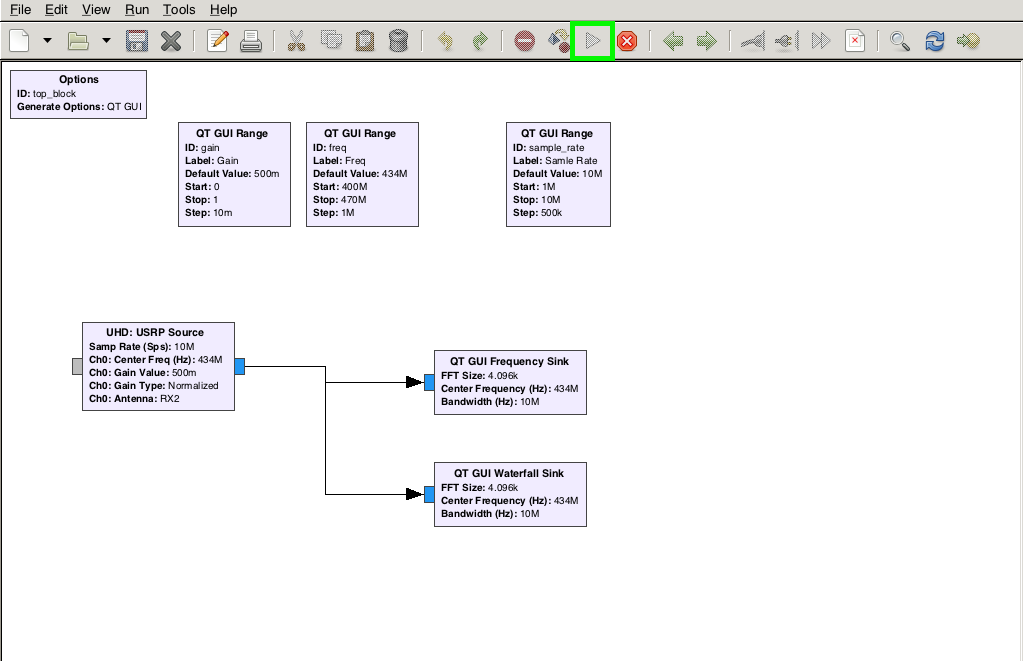
\includegraphics[width=\textwidth]{grc_fft.png}
\caption{gnuradio flow for viewing the spectrum}
\label{grc_fft}
\centrefigureend
\newpage

\section{Sending a secret message}
In this section we will use our feathers to send some messages to each other. Fortunately this is pretty simple to get started with thanks to the code provided by the RadioHead-Extras library provided.
For further information on Arduino libraries consult the Arduino website\footnote{\url{https://www.arduino.cc/en/Main/Libraries}}

\cfbox{red}{ Open up the provided SimpleFSKSend.ino sketch and the SimpleFSKRx.ino files in the Arduino editor and load them on to different feathers. } 

You should see that one is sending a message and the other is receiving it, and printing it to the serial monitor. This is our secret message! Try changing the code to send another message but for now keep the settings of the \gls{RF} chip the same, we will come back and change them later.
\newpage

\section{Spying on a secret message}
gnuradio
\newpage

\section{Real World Examples and Further Projects}
\subsection{Tyre Pressure Monitoring System}
This technique can be used in the 'real world' as demonstrated here: \url{https://www.sharebrained.com/downloads/toorcon/dude\_wheres\_my\_car\_toorcon\_sd\_2013.pdf} where someone has used the same technology to find out the tyre pressure of different cars near them. Work through the slides and the code provided and see what you can see.

\subsection{FM Reciever}
You can listen to the radio, and watch the spectrum and signals change as you do it by following the guide here: \url{https://www.instructables.com/id/RTL-SDR-FM-radio-receiver-with-GNU-Radio-Companion/}

\subsection{Satellite Images}
There is a rough guide for receiving images from weather satellites available which may require some special configuration of antenna, if you're up for it! 

\url{http://oz9aec.net/radios/gnu-radio/noaa-weather-satellite-reception-with-gnu-radio-and-usrp/}

\newpage

\end{document}
